% 2021-11-27
\begin{exercise}
      {ID-569cd24194aa27d54b34a2aefd1992510fedb32b}
      {Ortskurve der Wendepunkte}
  \ifproblem\problem\par
    % <PROBLEM>
    Gegeben sei die Funktionenschar
    $f_t:\mathbb{R}\to\mathbb{R}$ mit
    \begin{equation*}
      f_t(x)=\frac{1}{3}x^3-2tx^2
      \quad\text{und}\quad
      t\in\mathbb{R}.
    \end{equation*}
    Bestimmen Sie die Funktionsgleichung der
    Ortskurve $w(x)$, auf der sich die
    Wendepunkte aller Funktionen der
    Funktionenschar $f_t$ befinden.
    % </PROBLEM>
  \fi
  %\ifoutline\outline\par
    % <OUTLINE>
    % </OUTLINE>
  %\fi
  \ifoutcome\outcome\par
    % <OUTCOME>
    Als erstes müssen die Koordinaten des
    Wendepunktes $W$ ermittelt werden.
    Dazu behandelt man den Parameter $t$
    wie eine konstante (aber noch unbekannte)
    Zahl. Dabei ist es nicht unüblich, sondern
    eher zu erwarten, dass der Parameter $t$
    auch in der $x$- bzw. der $y$-Koordinate
    des Wendepunktes auftritt.
    \par
    Die ersten drei Ableitungen lauten:
    \begin{equation*}
        f_t(x)=\frac{1}{3}x^3-2tx^2
        \qquad
        f'_t(x)=x^2-4tx
        \qquad
        f''_t(x)=2x-4t
        \qquad
        f'''_t(x)=2
    \end{equation*}
    Notwendig für das Vorhandensein eines
    Wendepunktes in $f$ ist eine Nullstelle
    in der zweiten Ableitung $f''$, also:
    \begin{alignat*}{3}
      \relax&\quad
      &
      f''_t(x)=0&=2x-4t
      &
      \quad&|+4t
      \\
      \Leftrightarrow&\quad
      &
      4t&=2x
      &
      \quad&|:2
      \\
      \Leftrightarrow&\quad
      &
      2t&=x
      &
      \quad&\relax
    \end{alignat*}
    Wenn darüber hinaus sichergestellt ist,
    dass die dritte Ableitung $f'''$ an dieser
    Stelle nicht den Wert Null annimmt, hat
    man zweifelsfrei die $x$-Koordinate eines
    Wendepunktes von $f$ ermittelt.
    \begin{equation*}
      f'''_t(2t)=2\neq0
    \end{equation*}
    Also ist $2t$ tatsächlich die $x$-Koordinate
    eines Wendepunktes von $f_t$.
    Die $y$-Koordinate des Wendepunktes erhält
    man, indem man $2t$ für $x$ in $f_t(x)$
    einsetzt:
    \begin{equation*}
      \begin{split}
        f_t(2t)&=\frac{1}{3}\cdot(2t)^3-2t\cdot(2t)^2
        \\[1ex]
        &=\frac{1}{3}\cdot8t^3-2t\cdot4t^2
        \\[1ex]
        &=\frac{8}{3}t^3-8t^3
        \\[1ex]
        &=\left(\frac{8}{3}-8\right)\cdot t^3
        \\[1ex]
        &=\left(\frac{8}{3}-\frac{24}{3}\right)\cdot t^3
         =-\frac{16}{3}t^3
      \end{split}
    \end{equation*}
    Jede Funktion der Funktionenschar $f_t$ besitzt
    also genau einen Wendepunkt $W$ mit den
    Koordinaten:
    \begin{equation*}
      W\left(2t\;\middle|\;-\frac{16}{3}t^3\right)
    \end{equation*}
    Für jede Wahl von $t$ kann man damit also die
    beiden Koordinaten des jeweiligen Wendepunktes
    bestimmen.
    Nun fragt man sich aber nicht mehr, wo der
    Wendepunkt liegt, wenn man ein bestimmtes
    $t$ wählt, sondern welches $t$ man wählen
    muss, damit der Wendepunkt an einer
    gewählten Stelle $x$ liegt (und welches
    $y$ sich dort ergibt).
    Diese Fragestellung führt auf die
    Funktionsgleichung der Ortskurve der
    Wendepunkte von $f_t$ in Abhängigkeit
    von $x$.
    \par
    Im vorliegenden Fall gilt für die
    Koordinaten der Wendepunkte:
    \begin{equation*}
      x=2t
      \qquad
      y=-\frac{16}{3}t^3
    \end{equation*}
    Um das passende $t$ zu finden, für das
    der Wendepunkt an der Stelle $x$ liegt,
    löst man einfach die Gleichung der
    $x$-Ko\-or\-di\-na\-te nach $t$ auf:
    \begin{equation*}
      x=2t
      \quad\Rightarrow\quad
      t=\frac{x}{2}
    \end{equation*}
    Mit diesem $t$ erhält man die $y$-Koordinate
    des Wendepunktes an der Stelle $x$:
    \begin{equation*}
      y=-\frac{16}{3}t^3
       =-\frac{16}{3}\cdot\left(\frac{x}{2}\right)^3
       =-\frac{16}{3}\cdot\frac{x^3}{8}
       =-\frac{2}{3}x^3
    \end{equation*}
    Die Ortskurve der Wendepunkte von $f_t$ ist
    also der Graph der Funktion:
    \begin{equation*}
      w(x)=-\frac{2}{3}x^3
    \end{equation*}
    \begin{center}
      %<OCTAVE>
      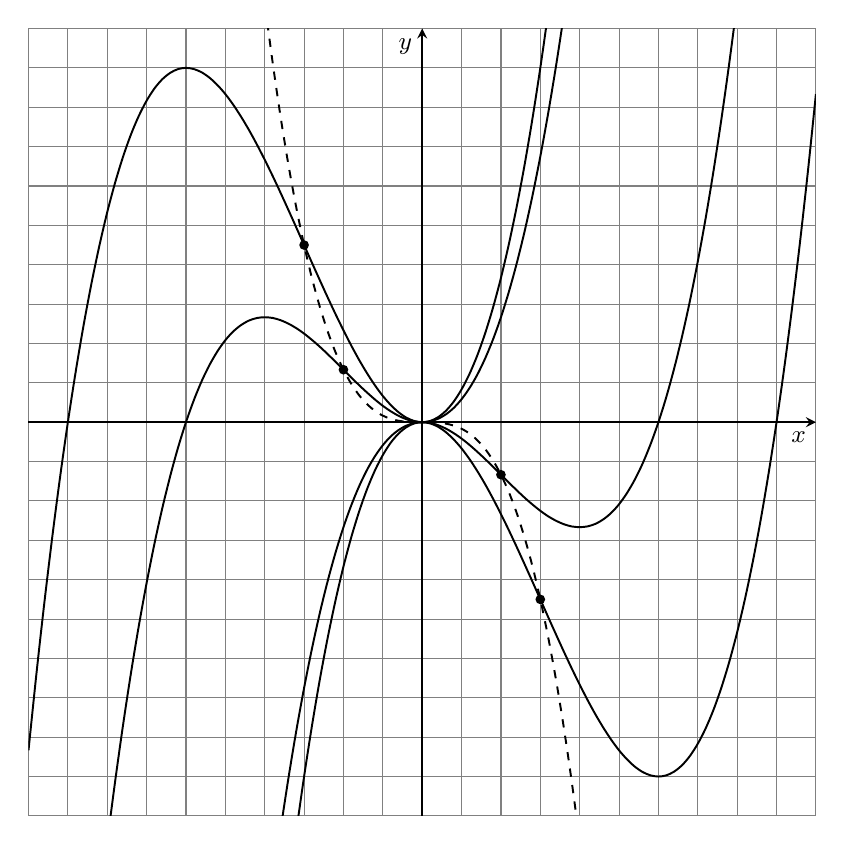
\begin{tikzpicture}[scale=1.000]
        % grid
        \draw[draw=black!50!white] (-5.000, -5.000) grid[step=0.5] (5.000, 5.000);
        % x-axis
        \draw[line width=0.6pt, ->, >=stealth] (-5.000, 0) -- (5.000, 0) node[below left] {\small$x$};
        % y-axis
        \draw[line width=0.6pt, ->, >=stealth] (0, -5.000) -- (0, 5.000) node[below left] {\small$y$};
        % function: f(x)=-\num{0.6666667}x^{3}
        \begin{scope}[line width=0.7pt]
          \clip (-5.000, -5.000) rectangle (5.000, 5.000);
          \draw[style=dashed] plot[smooth] coordinates
          {
            ( -5.000,   8.000) ( -4.900,   8.000) ( -4.800,   8.000)
            ( -4.700,   8.000) ( -4.600,   8.000) ( -4.500,   8.000)
            ( -4.400,   8.000) ( -4.300,   8.000) ( -4.200,   8.000)
            ( -4.100,   8.000) ( -4.000,   8.000) ( -3.900,   8.000)
            ( -3.800,   8.000) ( -3.700,   8.000) ( -3.600,   8.000)
            ( -3.500,   8.000) ( -3.400,   8.000) ( -3.300,   8.000)
            ( -3.200,   8.000) ( -3.100,   8.000) ( -3.000,   8.000)
            ( -2.900,   8.000) ( -2.800,   8.000) ( -2.700,   8.000)
            ( -2.600,   8.000) ( -2.500,   8.000) ( -2.400,   8.000)
            ( -2.300,   8.000) ( -2.200,   7.099) ( -2.100,   6.174)
            ( -2.000,   5.333) ( -1.900,   4.573) ( -1.800,   3.888)
            ( -1.700,   3.275) ( -1.600,   2.731) ( -1.500,   2.250)
            ( -1.400,   1.829) ( -1.300,   1.465) ( -1.200,   1.152)
            ( -1.100,   0.887) ( -1.000,   0.667) ( -0.900,   0.486)
            ( -0.800,   0.341) ( -0.700,   0.229) ( -0.600,   0.144)
            ( -0.500,   0.083) ( -0.400,   0.043) ( -0.300,   0.018)
            ( -0.200,   0.005) ( -0.100,   0.001) (  0.000,   0.000)
            (  0.100,  -0.001) (  0.200,  -0.005) (  0.300,  -0.018)
            (  0.400,  -0.043) (  0.500,  -0.083) (  0.600,  -0.144)
            (  0.700,  -0.229) (  0.800,  -0.341) (  0.900,  -0.486)
            (  1.000,  -0.667) (  1.100,  -0.887) (  1.200,  -1.152)
            (  1.300,  -1.465) (  1.400,  -1.829) (  1.500,  -2.250)
            (  1.600,  -2.731) (  1.700,  -3.275) (  1.800,  -3.888)
            (  1.900,  -4.573) (  2.000,  -5.333) (  2.100,  -6.174)
            (  2.200,  -7.099) (  2.300,  -8.000) (  2.400,  -8.000)
            (  2.500,  -8.000) (  2.600,  -8.000) (  2.700,  -8.000)
            (  2.800,  -8.000) (  2.900,  -8.000) (  3.000,  -8.000)
            (  3.100,  -8.000) (  3.200,  -8.000) (  3.300,  -8.000)
            (  3.400,  -8.000) (  3.500,  -8.000) (  3.600,  -8.000)
            (  3.700,  -8.000) (  3.800,  -8.000) (  3.900,  -8.000)
            (  4.000,  -8.000) (  4.100,  -8.000) (  4.200,  -8.000)
            (  4.300,  -8.000) (  4.400,  -8.000) (  4.500,  -8.000)
            (  4.600,  -8.000) (  4.700,  -8.000) (  4.800,  -8.000)
            (  4.900,  -8.000) (  5.000,  -8.000)
          };
        \end{scope}
        % function: f(x)=\num{0.3333333}x^{3}-x^{2}
        \begin{scope}[line width=0.7pt]
          \clip (-5.000, -5.000) rectangle (5.000, 5.000);
          \draw plot[smooth] coordinates
          {
            ( -5.000,  -8.000) ( -4.900,  -8.000) ( -4.800,  -8.000)
            ( -4.700,  -8.000) ( -4.600,  -8.000) ( -4.500,  -8.000)
            ( -4.400,  -8.000) ( -4.300,  -8.000) ( -4.200,  -8.000)
            ( -4.100,  -8.000) ( -4.000,  -8.000) ( -3.900,  -8.000)
            ( -3.800,  -8.000) ( -3.700,  -8.000) ( -3.600,  -8.000)
            ( -3.500,  -8.000) ( -3.400,  -8.000) ( -3.300,  -8.000)
            ( -3.200,  -8.000) ( -3.100,  -8.000) ( -3.000,  -8.000)
            ( -2.900,  -8.000) ( -2.800,  -8.000) ( -2.700,  -8.000)
            ( -2.600,  -8.000) ( -2.500,  -8.000) ( -2.400,  -8.000)
            ( -2.300,  -8.000) ( -2.200,  -8.000) ( -2.100,  -7.497)
            ( -2.000,  -6.667) ( -1.900,  -5.896) ( -1.800,  -5.184)
            ( -1.700,  -4.528) ( -1.600,  -3.925) ( -1.500,  -3.375)
            ( -1.400,  -2.875) ( -1.300,  -2.422) ( -1.200,  -2.016)
            ( -1.100,  -1.654) ( -1.000,  -1.333) ( -0.900,  -1.053)
            ( -0.800,  -0.811) ( -0.700,  -0.604) ( -0.600,  -0.432)
            ( -0.500,  -0.292) ( -0.400,  -0.181) ( -0.300,  -0.099)
            ( -0.200,  -0.043) ( -0.100,  -0.010) (  0.000,   0.000)
            (  0.100,  -0.010) (  0.200,  -0.037) (  0.300,  -0.081)
            (  0.400,  -0.139) (  0.500,  -0.208) (  0.600,  -0.288)
            (  0.700,  -0.376) (  0.800,  -0.469) (  0.900,  -0.567)
            (  1.000,  -0.667) (  1.100,  -0.766) (  1.200,  -0.864)
            (  1.300,  -0.958) (  1.400,  -1.045) (  1.500,  -1.125)
            (  1.600,  -1.195) (  1.700,  -1.252) (  1.800,  -1.296)
            (  1.900,  -1.324) (  2.000,  -1.333) (  2.100,  -1.323)
            (  2.200,  -1.291) (  2.300,  -1.234) (  2.400,  -1.152)
            (  2.500,  -1.042) (  2.600,  -0.901) (  2.700,  -0.729)
            (  2.800,  -0.523) (  2.900,  -0.280) (  3.000,   0.000)
            (  3.100,   0.320) (  3.200,   0.683) (  3.300,   1.089)
            (  3.400,   1.541) (  3.500,   2.042) (  3.600,   2.592)
            (  3.700,   3.194) (  3.800,   3.851) (  3.900,   4.563)
            (  4.000,   5.333) (  4.100,   6.164) (  4.200,   7.056)
            (  4.300,   8.000) (  4.400,   8.000) (  4.500,   8.000)
            (  4.600,   8.000) (  4.700,   8.000) (  4.800,   8.000)
            (  4.900,   8.000) (  5.000,   8.000)
          };
        \end{scope}
        % function: f(x)=\num{0.3333333}x^{3}-\num{1.5}x^{2}
        \begin{scope}[line width=0.7pt]
          \clip (-5.000, -5.000) rectangle (5.000, 5.000);
          \draw plot[smooth] coordinates
          {
            ( -5.000,  -8.000) ( -4.900,  -8.000) ( -4.800,  -8.000)
            ( -4.700,  -8.000) ( -4.600,  -8.000) ( -4.500,  -8.000)
            ( -4.400,  -8.000) ( -4.300,  -8.000) ( -4.200,  -8.000)
            ( -4.100,  -8.000) ( -4.000,  -8.000) ( -3.900,  -8.000)
            ( -3.800,  -8.000) ( -3.700,  -8.000) ( -3.600,  -8.000)
            ( -3.500,  -8.000) ( -3.400,  -8.000) ( -3.300,  -8.000)
            ( -3.200,  -8.000) ( -3.100,  -8.000) ( -3.000,  -8.000)
            ( -2.900,  -8.000) ( -2.800,  -8.000) ( -2.700,  -8.000)
            ( -2.600,  -8.000) ( -2.500,  -8.000) ( -2.400,  -8.000)
            ( -2.300,  -8.000) ( -2.200,  -8.000) ( -2.100,  -8.000)
            ( -2.000,  -8.000) ( -1.900,  -7.701) ( -1.800,  -6.804)
            ( -1.700,  -5.973) ( -1.600,  -5.205) ( -1.500,  -4.500)
            ( -1.400,  -3.855) ( -1.300,  -3.267) ( -1.200,  -2.736)
            ( -1.100,  -2.259) ( -1.000,  -1.833) ( -0.900,  -1.458)
            ( -0.800,  -1.131) ( -0.700,  -0.849) ( -0.600,  -0.612)
            ( -0.500,  -0.417) ( -0.400,  -0.261) ( -0.300,  -0.144)
            ( -0.200,  -0.063) ( -0.100,  -0.015) (  0.000,   0.000)
            (  0.100,  -0.015) (  0.200,  -0.057) (  0.300,  -0.126)
            (  0.400,  -0.219) (  0.500,  -0.333) (  0.600,  -0.468)
            (  0.700,  -0.621) (  0.800,  -0.789) (  0.900,  -0.972)
            (  1.000,  -1.167) (  1.100,  -1.371) (  1.200,  -1.584)
            (  1.300,  -1.803) (  1.400,  -2.025) (  1.500,  -2.250)
            (  1.600,  -2.475) (  1.700,  -2.697) (  1.800,  -2.916)
            (  1.900,  -3.129) (  2.000,  -3.333) (  2.100,  -3.528)
            (  2.200,  -3.711) (  2.300,  -3.879) (  2.400,  -4.032)
            (  2.500,  -4.167) (  2.600,  -4.281) (  2.700,  -4.374)
            (  2.800,  -4.443) (  2.900,  -4.485) (  3.000,  -4.500)
            (  3.100,  -4.485) (  3.200,  -4.437) (  3.300,  -4.356)
            (  3.400,  -4.239) (  3.500,  -4.083) (  3.600,  -3.888)
            (  3.700,  -3.651) (  3.800,  -3.369) (  3.900,  -3.042)
            (  4.000,  -2.667) (  4.100,  -2.241) (  4.200,  -1.764)
            (  4.300,  -1.233) (  4.400,  -0.645) (  4.500,   0.000)
            (  4.600,   0.705) (  4.700,   1.473) (  4.800,   2.304)
            (  4.900,   3.201) (  5.000,   4.167)
          };
        \end{scope}
        % function: f(x)=\num{0.3333333}x^{3}+x^{2}
        \begin{scope}[line width=0.7pt]
          \clip (-5.000, -5.000) rectangle (5.000, 5.000);
          \draw plot[smooth] coordinates
          {
            ( -5.000,  -8.000) ( -4.900,  -8.000) ( -4.800,  -8.000)
            ( -4.700,  -8.000) ( -4.600,  -8.000) ( -4.500,  -8.000)
            ( -4.400,  -8.000) ( -4.300,  -8.000) ( -4.200,  -7.056)
            ( -4.100,  -6.164) ( -4.000,  -5.333) ( -3.900,  -4.563)
            ( -3.800,  -3.851) ( -3.700,  -3.194) ( -3.600,  -2.592)
            ( -3.500,  -2.042) ( -3.400,  -1.541) ( -3.300,  -1.089)
            ( -3.200,  -0.683) ( -3.100,  -0.320) ( -3.000,   0.000)
            ( -2.900,   0.280) ( -2.800,   0.523) ( -2.700,   0.729)
            ( -2.600,   0.901) ( -2.500,   1.042) ( -2.400,   1.152)
            ( -2.300,   1.234) ( -2.200,   1.291) ( -2.100,   1.323)
            ( -2.000,   1.333) ( -1.900,   1.324) ( -1.800,   1.296)
            ( -1.700,   1.252) ( -1.600,   1.195) ( -1.500,   1.125)
            ( -1.400,   1.045) ( -1.300,   0.958) ( -1.200,   0.864)
            ( -1.100,   0.766) ( -1.000,   0.667) ( -0.900,   0.567)
            ( -0.800,   0.469) ( -0.700,   0.376) ( -0.600,   0.288)
            ( -0.500,   0.208) ( -0.400,   0.139) ( -0.300,   0.081)
            ( -0.200,   0.037) ( -0.100,   0.010) (  0.000,   0.000)
            (  0.100,   0.010) (  0.200,   0.043) (  0.300,   0.099)
            (  0.400,   0.181) (  0.500,   0.292) (  0.600,   0.432)
            (  0.700,   0.604) (  0.800,   0.811) (  0.900,   1.053)
            (  1.000,   1.333) (  1.100,   1.654) (  1.200,   2.016)
            (  1.300,   2.422) (  1.400,   2.875) (  1.500,   3.375)
            (  1.600,   3.925) (  1.700,   4.528) (  1.800,   5.184)
            (  1.900,   5.896) (  2.000,   6.667) (  2.100,   7.497)
            (  2.200,   8.000) (  2.300,   8.000) (  2.400,   8.000)
            (  2.500,   8.000) (  2.600,   8.000) (  2.700,   8.000)
            (  2.800,   8.000) (  2.900,   8.000) (  3.000,   8.000)
            (  3.100,   8.000) (  3.200,   8.000) (  3.300,   8.000)
            (  3.400,   8.000) (  3.500,   8.000) (  3.600,   8.000)
            (  3.700,   8.000) (  3.800,   8.000) (  3.900,   8.000)
            (  4.000,   8.000) (  4.100,   8.000) (  4.200,   8.000)
            (  4.300,   8.000) (  4.400,   8.000) (  4.500,   8.000)
            (  4.600,   8.000) (  4.700,   8.000) (  4.800,   8.000)
            (  4.900,   8.000) (  5.000,   8.000)
          };
        \end{scope}
        % function: f(x)=\num{0.3333333}x^{3}+\num{1.5}x^{2}
        \begin{scope}[line width=0.7pt]
          \clip (-5.000, -5.000) rectangle (5.000, 5.000);
          \draw plot[smooth] coordinates
          {
            ( -5.000,  -4.167) ( -4.900,  -3.201) ( -4.800,  -2.304)
            ( -4.700,  -1.473) ( -4.600,  -0.705) ( -4.500,   0.000)
            ( -4.400,   0.645) ( -4.300,   1.233) ( -4.200,   1.764)
            ( -4.100,   2.241) ( -4.000,   2.667) ( -3.900,   3.042)
            ( -3.800,   3.369) ( -3.700,   3.651) ( -3.600,   3.888)
            ( -3.500,   4.083) ( -3.400,   4.239) ( -3.300,   4.356)
            ( -3.200,   4.437) ( -3.100,   4.485) ( -3.000,   4.500)
            ( -2.900,   4.485) ( -2.800,   4.443) ( -2.700,   4.374)
            ( -2.600,   4.281) ( -2.500,   4.167) ( -2.400,   4.032)
            ( -2.300,   3.879) ( -2.200,   3.711) ( -2.100,   3.528)
            ( -2.000,   3.333) ( -1.900,   3.129) ( -1.800,   2.916)
            ( -1.700,   2.697) ( -1.600,   2.475) ( -1.500,   2.250)
            ( -1.400,   2.025) ( -1.300,   1.803) ( -1.200,   1.584)
            ( -1.100,   1.371) ( -1.000,   1.167) ( -0.900,   0.972)
            ( -0.800,   0.789) ( -0.700,   0.621) ( -0.600,   0.468)
            ( -0.500,   0.333) ( -0.400,   0.219) ( -0.300,   0.126)
            ( -0.200,   0.057) ( -0.100,   0.015) (  0.000,   0.000)
            (  0.100,   0.015) (  0.200,   0.063) (  0.300,   0.144)
            (  0.400,   0.261) (  0.500,   0.417) (  0.600,   0.612)
            (  0.700,   0.849) (  0.800,   1.131) (  0.900,   1.458)
            (  1.000,   1.833) (  1.100,   2.259) (  1.200,   2.736)
            (  1.300,   3.267) (  1.400,   3.855) (  1.500,   4.500)
            (  1.600,   5.205) (  1.700,   5.973) (  1.800,   6.804)
            (  1.900,   7.701) (  2.000,   8.000) (  2.100,   8.000)
            (  2.200,   8.000) (  2.300,   8.000) (  2.400,   8.000)
            (  2.500,   8.000) (  2.600,   8.000) (  2.700,   8.000)
            (  2.800,   8.000) (  2.900,   8.000) (  3.000,   8.000)
            (  3.100,   8.000) (  3.200,   8.000) (  3.300,   8.000)
            (  3.400,   8.000) (  3.500,   8.000) (  3.600,   8.000)
            (  3.700,   8.000) (  3.800,   8.000) (  3.900,   8.000)
            (  4.000,   8.000) (  4.100,   8.000) (  4.200,   8.000)
            (  4.300,   8.000) (  4.400,   8.000) (  4.500,   8.000)
            (  4.600,   8.000) (  4.700,   8.000) (  4.800,   8.000)
            (  4.900,   8.000) (  5.000,   8.000)
          };
        \end{scope}
        \fill (1.0000, -0.6667) circle[radius=1.75pt];
        \fill (1.5000, -2.2500) circle[radius=1.75pt];
        \fill (-1.0000, 0.6667) circle[radius=1.75pt];
        \fill (-1.5000, 2.2500) circle[radius=1.75pt];
        %t = -0.75;
        %x = 2 * t;
        %y = -2/3 * x^3;
        %printf("\\fill (%6.4f, %6.4f) circle[radius=1.75pt];\n", x, y);
      \end{tikzpicture}
      %</OCTAVE>
      %w = [-2/3 0 0 0];
      %mypolyplot(w, -5, 5, -5, 5, 0.1)
      %t = 0.5;
      %f = [1/3 -2*t 0 0];
      %mypolyplot(f, -5, 5, -5, 5, 0.1)
      %t = 0.75;
      %f = [1/3 -2*t 0 0];
      %mypolyplot(f, -5, 5, -5, 5, 0.1)
      %t = -0.5;
      %f = [1/3 -2*t 0 0];
      %mypolyplot(f, -5, 5, -5, 5, 0.1)
      %t = -0.75;
      %f = [1/3 -2*t 0 0];
      %mypolyplot(f, -5, 5, -5, 5, 0.1)
    \end{center}
    % </OUTCOME>
  \fi
\end{exercise}
